% Appendix A

\chapter{Organisation des types d'expérimentations} % Main appendix title

\label{AppendixC} % For referencing this appendix elsewhere, use \ref{AppendixC}



Pour une question de clarté, nous avons jugé nécessaire de décrire comment est organisé chaque type d'expérimentation avons de passer aux résultats obtenus.

\section{Expérimentation par rapport à la portée des cibles}
Pour les expérimentations par rapport à l'influence de la portée des cibles sur le comportement de nos algorithmes de recherche, nous avons fixé la taille de l'environnement à 500 $\times$ 500 positions et fait varier la portée d'un rayon de 10 positions à 100 positions avec un pas de 10.

Ainsi comme le montre la figure \ref{orgPortee}, les tests de ce type proviennent des exécutions sur 40 environnements (4 par portée), soit 400 exécutions pour le mono-cible et 400 autres pour le multi-cible, pour chaque méta-heuristique (après paramétrage).

\begin{center}	 
	\captionsetup{width=1\linewidth} 
	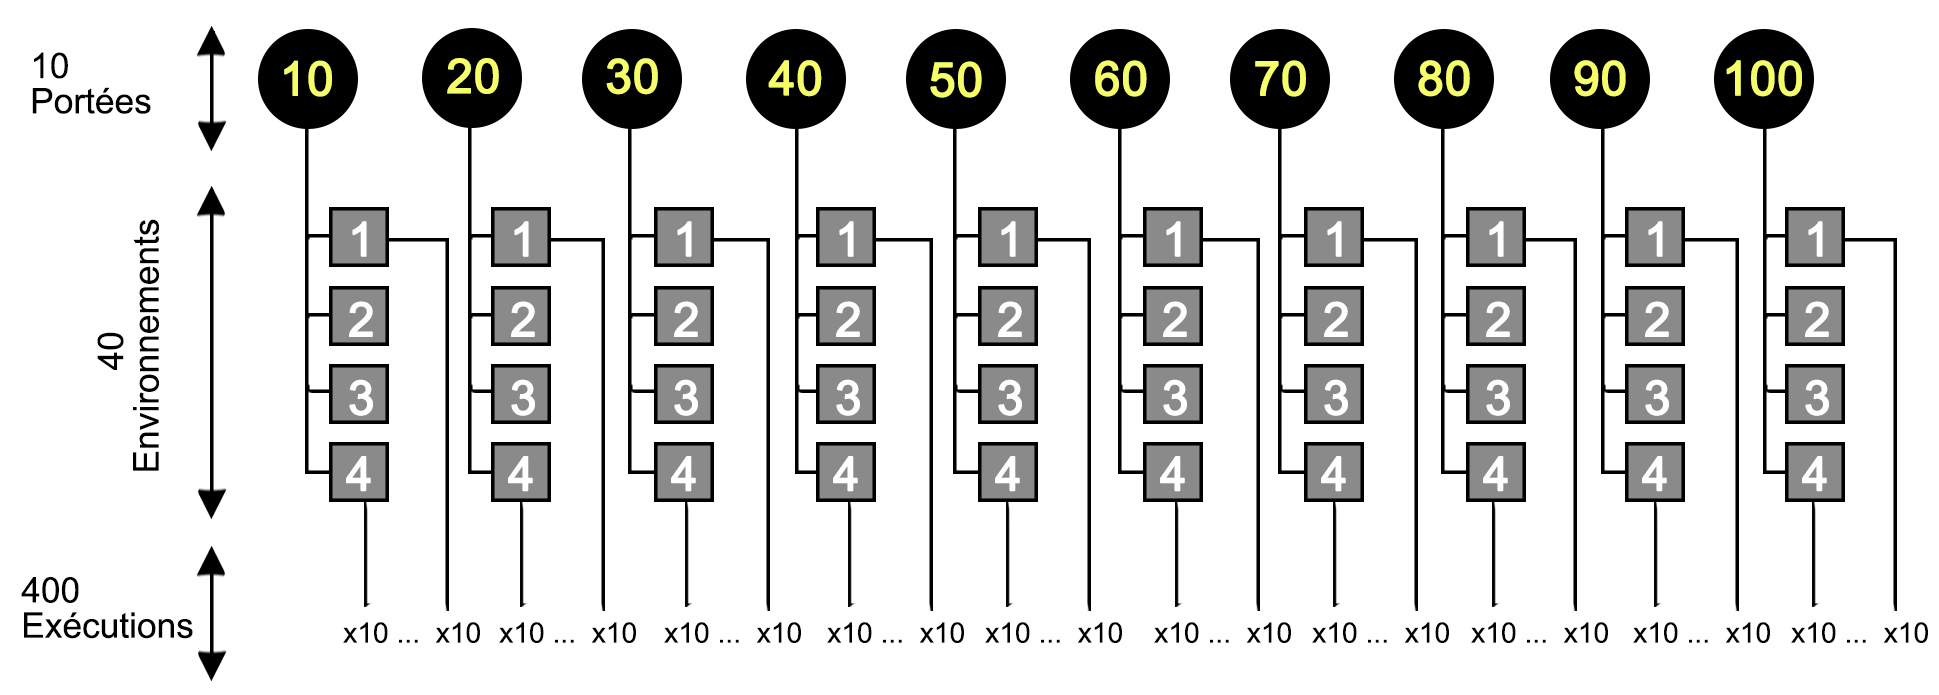
\includegraphics[width=0.7\textwidth]{org-portee.jpg}%
	\vspace{-0.1 cm}
	\captionof{figure}{Représentation de l'organisation des expérimentations sur la portée des cibles.}\label{orgPortee}%
\end{center}

\section{Expérimentation par rapport à la taille de l'environnement}
Pour les expérimentations sur l'influence de la taille de l'environnement sur le comportement de nos méta-heuristiques pour la recherche de cibles, nous avons adapté la portée des cibles à chaque taille d'environnement conformément à l'équation suivante:
\begin{equation}
portee = \frac{taille_{Cot\acute{e}} \times 10}{100} = \frac{taille_{Cot\acute{e}}}{10}
\label{porteeEnv}
\end{equation}	
Ce qui revient à :
\begin{equation}	
S_{cible} = \frac{\sqrt{S_{env}}}{5} \times \pi
\end{equation}

Avec :
\begin{itemize}
	\item[$-$] $taille_{Cot\acute{e}}$ : taille du coté de l'environnement carré.
	\item[$-$] $S_{cible}$ : surface d'émission de la cible (rayon = portée).
	\item[$-$] $S_{env}$ : surface de l'environnement de recherche ($S_{env}$ = $taille_{Cot\acute{e}}$).\\
\end{itemize}

Pour cela nous avons sélectionné dix différentes tailles d'environnement, les tailles du coté de ces environnements sont comme suit : 50, 100, 200, 400, 600, 800, 1000, 1500, 3000, 5000.

les surfaces respectives sont les suivantes: 2500, 10000, 40000, 160000, 360000, 640000, 1000000, 2250000, 9000000, 25000000.

Ainsi les portées correspondantes sont: 5, 10, 20, 40, 60, 80, 100, 150, 300, 500.


\textbf{ }\\
Les résultats des testes liés à ce type sont le résultat de 40 exécutions par taille d'environnement (4 configurations pour chaque taille), ce qui revient à un total de 400 exécutions pour le mono-cible et 400 autres pour le multi-cible, et ce pour chaque approche (après paramétrage). Le schéma \ref{orgSize} ci-dessous illustre cette organisation.

\begin{center}	  
	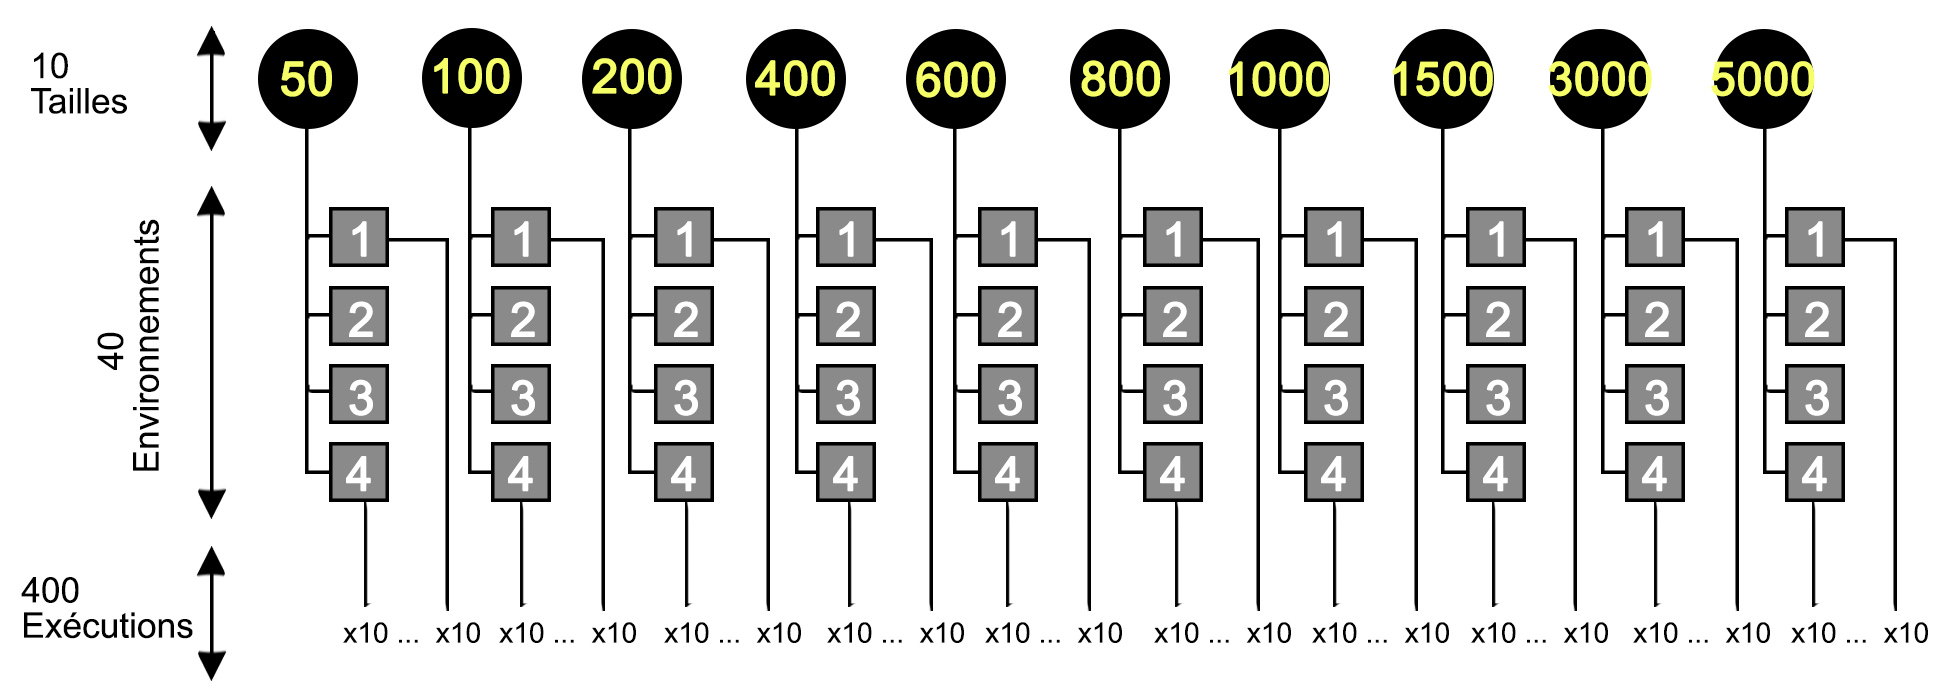
\includegraphics[width=0.75\textwidth]{org-size.jpg}%
	\vspace{-0.1 cm}
	\captionof{figure}{Représentation de l'organisation des expérimentations sur la taille des environnements.}\label{orgSize}%
\end{center}

\section{Expérimentation par rapport au nombre de cible}
Ces expérimentations permettent d'étudier l'influence du nombre de cibles présentes dans nos environnements sur le comportement de nos métaheuristiques (BSO, EHO, ESWSA et MBSO).
Pour cela nous avons fixé la taille des environnements à 500 $\times$ 500 positions ainsi qu'une portée de cible égale à 50 (conformément à l'équation \ref{porteeEnv}).\\

Nous avons pris le nombre de variable compris entre 1 et 15 (bornes incluent) avec un pas de 2, ce qui nous donne les 8 nombres de cibles suivants : 1, 3, 5, 7, 9, 11, 13, 15.\\

De ce fait, les résultats des tests sont le fruit d'exécution sur 32 environnements (4 par nombre de cible) , ce qui correspond à 320 exécutions pour chacune des approches développées (après paramétrage).\\
La figure \ref{orgNbrT} ci-dessous schématise cette organisation:

\begin{center}	  
	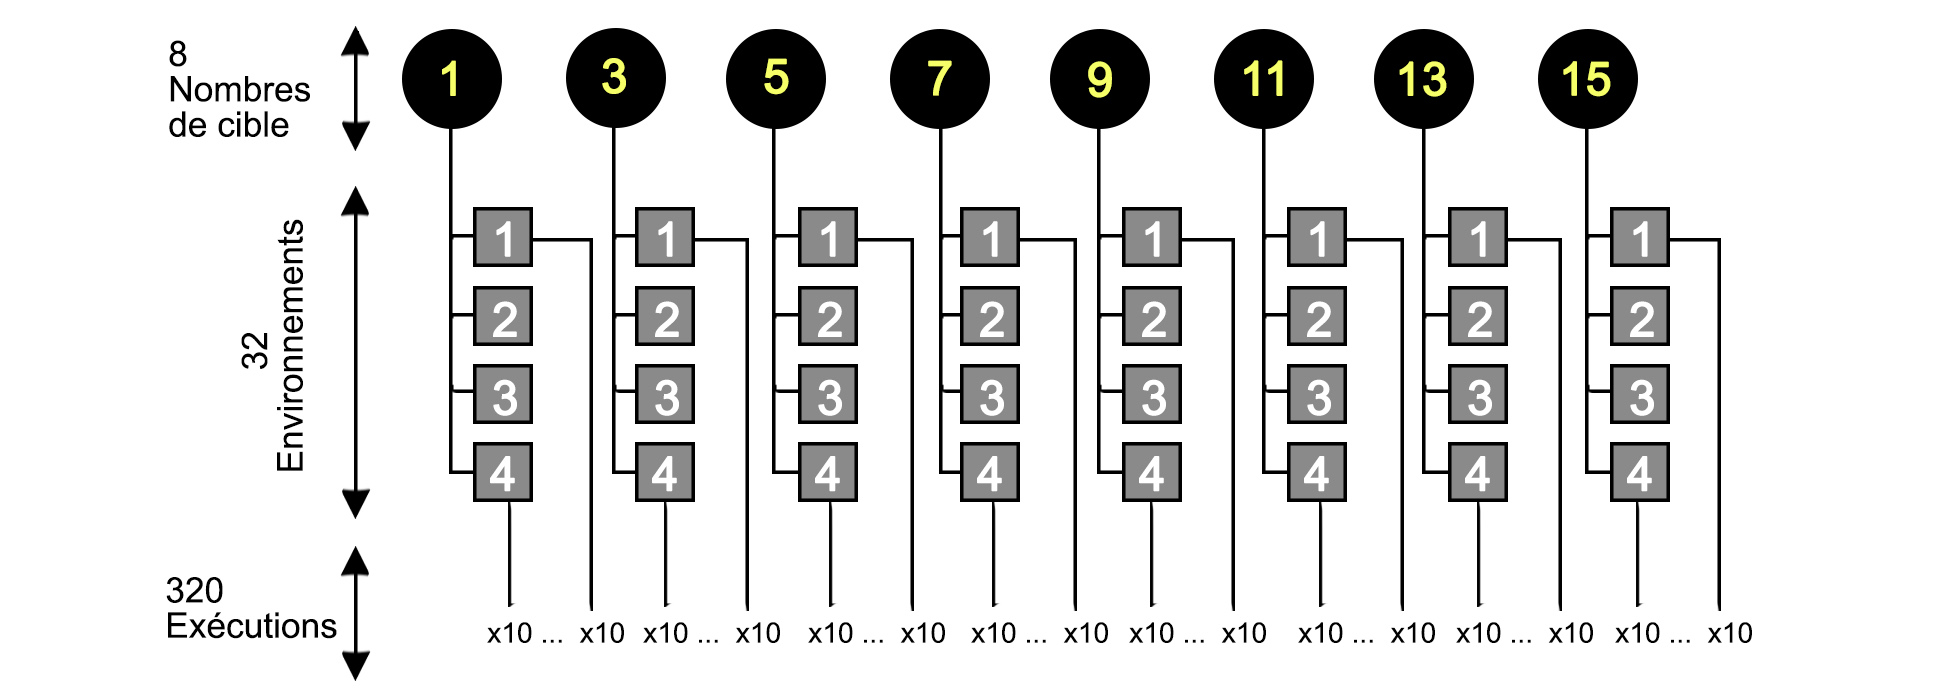
\includegraphics[width=0.8\textwidth]{org-nbrT.jpg}%
	\vspace{-0.1 cm}
	\captionof{figure}{Représentation de l'organisation des expérimentations sur le nombre de cible.}\label{orgNbrT}%
\end{center}
